\sect{Конструкторская часть}
\label{cha:design}

В данном разделе приведены схемы алгоритмов решения задачи коммивояжера: полным перебором и на основе муравьиного алгоритма. 
Также приведена оценка трудоёмкости рассмотренных алгоритмов.

%=====================================================================
\subsect{Разработка алгоритмов}

На рисунке~\ref{fig:full-comb} представлена схема алгоритма полного перебора.
На рисунке~\ref{fig:ants} представлена схема муравьиного алгоритма.

\renewcommand{\thefigure}{\thesubsection.\arabic{figure}}
\begin{figure}[h]
	\centering
	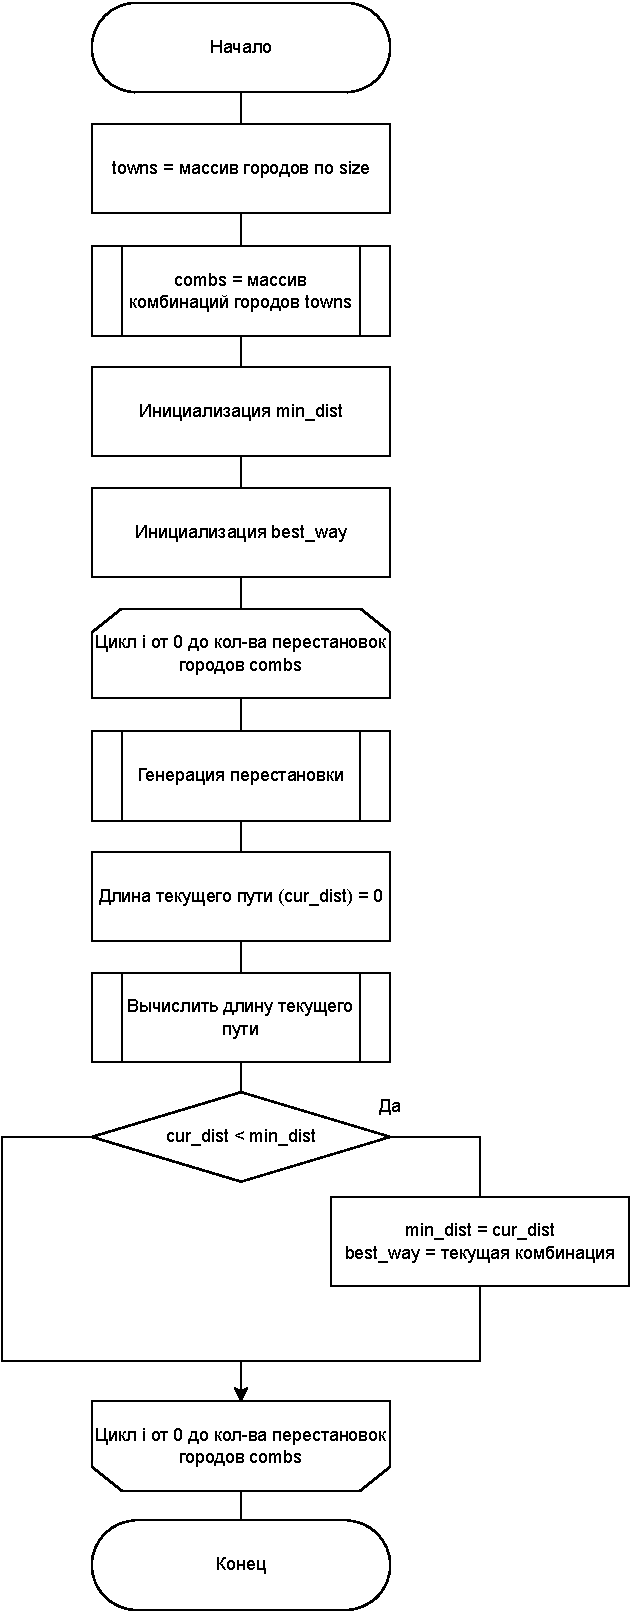
\includegraphics[height=0.9\textheight]{svg/all_combs}
	\caption{Схема алгоритма полного перебора}
	\label{fig:full-comb}
\end{figure}

\begin{figure}[h]
	\centering
	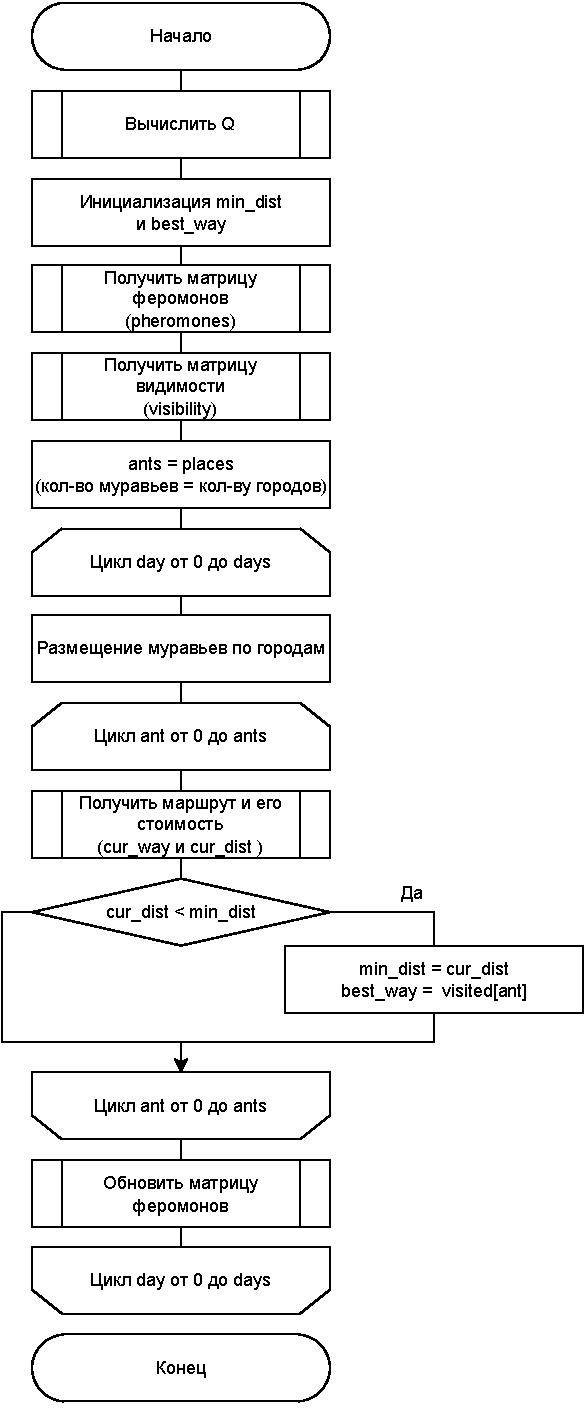
\includegraphics[height=0.9\textheight]{svg/ants}
	\caption{Схема алгоритма полного перебора}
	\label{fig:ants}
\end{figure}

%=====================================================================================
%\subsect{Модель вычислений}
%Для вычисления трудоемкости алгоритмов сортировок необходимо ввести следующую модель вычислений:
%\begin{enumerate}
%	\item Операции (\ref{for:opers}) имеют трудоемкость 1.
%		\begin{equation}
%			\label{for:opers}
%			=, +=, -=, +, -, ==, !=, <, >, <=, >=, [], ++, {-}-
%		\end{equation}
%
%	\item Операции (\ref{for:opers2}) имеют трудоемкость 2.
%		\begin{equation}
%			\label{for:opers2}
%			*, /, \%, *=, /=, \%=
%		\end{equation}
%	\item трудоемкость условного оператора рассчитывается согласно формуле (\ref{for:if});
%	\begin{equation}
%		\label{for:if}
%		f_{if} = f_{\text{условия}} +
%		\begin{cases}
%			f_A, & \text{если условие выполняется,}\\
%			f_B, & \text{иначе.}
%		\end{cases}
%	\end{equation}
%	\item трудоемкость цикла рассчитывается согласно формуле (\ref{for:for});
%	\begin{equation}
%		\label{for:for}
%		f_{for} = f_{\text{инициализации}} + f_{\text{сравнения}} + N(f_{\text{тела}} + f_{\text{инкремента}} + f_{\text{сравнения}})
%	\end{equation}
%	\item трудоемкость вызова функции принимается равной 0.
%\end{enumerate}

%=====================================================================================
%\subsect{Оценка трудоемкости алгоритма полного перебора}
%Трудоемкость цикла по всем возможным перестановкам вершин графа вычисляется по формуле~\ref{for:all_combs1}
%\begin{equation}
%	\label{for:all_combs1}
%	f = 1 + 1 + n!(1 + 1 + f_{body}) = 2 + n!(2 + f_{body})
%\end{equation}
%
%\begin{equation}
%	\label{for:all_combs2}
%	f_{body} = 3 + (n - 1)(3 + f_{if})
%\end{equation}

%=====================================================================================  
%\subsect{Оценка трудоемкости муравьиного алгоритма}


%#########################################################################
%\parag
